% Options for packages loaded elsewhere
\PassOptionsToPackage{unicode}{hyperref}
\PassOptionsToPackage{hyphens}{url}
%
\documentclass[
]{article}
\usepackage{amsmath,amssymb}
\usepackage{lmodern}
\usepackage{ifxetex,ifluatex}
\ifnum 0\ifxetex 1\fi\ifluatex 1\fi=0 % if pdftex
  \usepackage[T1]{fontenc}
  \usepackage[utf8]{inputenc}
  \usepackage{textcomp} % provide euro and other symbols
\else % if luatex or xetex
  \usepackage{unicode-math}
  \defaultfontfeatures{Scale=MatchLowercase}
  \defaultfontfeatures[\rmfamily]{Ligatures=TeX,Scale=1}
\fi
% Use upquote if available, for straight quotes in verbatim environments
\IfFileExists{upquote.sty}{\usepackage{upquote}}{}
\IfFileExists{microtype.sty}{% use microtype if available
  \usepackage[]{microtype}
  \UseMicrotypeSet[protrusion]{basicmath} % disable protrusion for tt fonts
}{}
\makeatletter
\@ifundefined{KOMAClassName}{% if non-KOMA class
  \IfFileExists{parskip.sty}{%
    \usepackage{parskip}
  }{% else
    \setlength{\parindent}{0pt}
    \setlength{\parskip}{6pt plus 2pt minus 1pt}}
}{% if KOMA class
  \KOMAoptions{parskip=half}}
\makeatother
\usepackage{xcolor}
\IfFileExists{xurl.sty}{\usepackage{xurl}}{} % add URL line breaks if available
\IfFileExists{bookmark.sty}{\usepackage{bookmark}}{\usepackage{hyperref}}
\hypersetup{
  pdftitle={Tarea1},
  pdfauthor={Gonzalo Ruiz Espinar},
  hidelinks,
  pdfcreator={LaTeX via pandoc}}
\urlstyle{same} % disable monospaced font for URLs
\usepackage[margin=1in]{geometry}
\usepackage{color}
\usepackage{fancyvrb}
\newcommand{\VerbBar}{|}
\newcommand{\VERB}{\Verb[commandchars=\\\{\}]}
\DefineVerbatimEnvironment{Highlighting}{Verbatim}{commandchars=\\\{\}}
% Add ',fontsize=\small' for more characters per line
\usepackage{framed}
\definecolor{shadecolor}{RGB}{248,248,248}
\newenvironment{Shaded}{\begin{snugshade}}{\end{snugshade}}
\newcommand{\AlertTok}[1]{\textcolor[rgb]{0.94,0.16,0.16}{#1}}
\newcommand{\AnnotationTok}[1]{\textcolor[rgb]{0.56,0.35,0.01}{\textbf{\textit{#1}}}}
\newcommand{\AttributeTok}[1]{\textcolor[rgb]{0.77,0.63,0.00}{#1}}
\newcommand{\BaseNTok}[1]{\textcolor[rgb]{0.00,0.00,0.81}{#1}}
\newcommand{\BuiltInTok}[1]{#1}
\newcommand{\CharTok}[1]{\textcolor[rgb]{0.31,0.60,0.02}{#1}}
\newcommand{\CommentTok}[1]{\textcolor[rgb]{0.56,0.35,0.01}{\textit{#1}}}
\newcommand{\CommentVarTok}[1]{\textcolor[rgb]{0.56,0.35,0.01}{\textbf{\textit{#1}}}}
\newcommand{\ConstantTok}[1]{\textcolor[rgb]{0.00,0.00,0.00}{#1}}
\newcommand{\ControlFlowTok}[1]{\textcolor[rgb]{0.13,0.29,0.53}{\textbf{#1}}}
\newcommand{\DataTypeTok}[1]{\textcolor[rgb]{0.13,0.29,0.53}{#1}}
\newcommand{\DecValTok}[1]{\textcolor[rgb]{0.00,0.00,0.81}{#1}}
\newcommand{\DocumentationTok}[1]{\textcolor[rgb]{0.56,0.35,0.01}{\textbf{\textit{#1}}}}
\newcommand{\ErrorTok}[1]{\textcolor[rgb]{0.64,0.00,0.00}{\textbf{#1}}}
\newcommand{\ExtensionTok}[1]{#1}
\newcommand{\FloatTok}[1]{\textcolor[rgb]{0.00,0.00,0.81}{#1}}
\newcommand{\FunctionTok}[1]{\textcolor[rgb]{0.00,0.00,0.00}{#1}}
\newcommand{\ImportTok}[1]{#1}
\newcommand{\InformationTok}[1]{\textcolor[rgb]{0.56,0.35,0.01}{\textbf{\textit{#1}}}}
\newcommand{\KeywordTok}[1]{\textcolor[rgb]{0.13,0.29,0.53}{\textbf{#1}}}
\newcommand{\NormalTok}[1]{#1}
\newcommand{\OperatorTok}[1]{\textcolor[rgb]{0.81,0.36,0.00}{\textbf{#1}}}
\newcommand{\OtherTok}[1]{\textcolor[rgb]{0.56,0.35,0.01}{#1}}
\newcommand{\PreprocessorTok}[1]{\textcolor[rgb]{0.56,0.35,0.01}{\textit{#1}}}
\newcommand{\RegionMarkerTok}[1]{#1}
\newcommand{\SpecialCharTok}[1]{\textcolor[rgb]{0.00,0.00,0.00}{#1}}
\newcommand{\SpecialStringTok}[1]{\textcolor[rgb]{0.31,0.60,0.02}{#1}}
\newcommand{\StringTok}[1]{\textcolor[rgb]{0.31,0.60,0.02}{#1}}
\newcommand{\VariableTok}[1]{\textcolor[rgb]{0.00,0.00,0.00}{#1}}
\newcommand{\VerbatimStringTok}[1]{\textcolor[rgb]{0.31,0.60,0.02}{#1}}
\newcommand{\WarningTok}[1]{\textcolor[rgb]{0.56,0.35,0.01}{\textbf{\textit{#1}}}}
\usepackage{graphicx}
\makeatletter
\def\maxwidth{\ifdim\Gin@nat@width>\linewidth\linewidth\else\Gin@nat@width\fi}
\def\maxheight{\ifdim\Gin@nat@height>\textheight\textheight\else\Gin@nat@height\fi}
\makeatother
% Scale images if necessary, so that they will not overflow the page
% margins by default, and it is still possible to overwrite the defaults
% using explicit options in \includegraphics[width, height, ...]{}
\setkeys{Gin}{width=\maxwidth,height=\maxheight,keepaspectratio}
% Set default figure placement to htbp
\makeatletter
\def\fps@figure{htbp}
\makeatother
\setlength{\emergencystretch}{3em} % prevent overfull lines
\providecommand{\tightlist}{%
  \setlength{\itemsep}{0pt}\setlength{\parskip}{0pt}}
\setcounter{secnumdepth}{-\maxdimen} % remove section numbering
\ifluatex
  \usepackage{selnolig}  % disable illegal ligatures
\fi

\title{Tarea1}
\author{Gonzalo Ruiz Espinar}
\date{9/15/2021}

\begin{document}
\maketitle

\hypertarget{ejercicio-0}{%
\subsubsection{Ejercicio 0}\label{ejercicio-0}}

Empezaremos cargamos la libreria \emph{tidyverse}.

\begin{Shaded}
\begin{Highlighting}[]
\FunctionTok{library}\NormalTok{(tidyverse)}
\end{Highlighting}
\end{Shaded}

Usando la función sample para crear un dado honesto con 100 números del
1 al 6.

\begin{Shaded}
\begin{Highlighting}[]
\NormalTok{dado\_honesto}\OtherTok{=}\FunctionTok{sample}\NormalTok{(}\DecValTok{1}\SpecialCharTok{:}\DecValTok{6}\NormalTok{, }\AttributeTok{size =} \DecValTok{100}\NormalTok{, }\AttributeTok{replace =} \ConstantTok{TRUE}\NormalTok{)}
\NormalTok{dado\_honesto}
\end{Highlighting}
\end{Shaded}

\begin{verbatim}
##   [1] 5 6 3 5 5 1 2 5 3 2 2 3 5 5 6 4 4 5 2 5 3 2 6 5 2 2 4 5 4 1 5 3 6 5 3 1 2
##  [38] 2 3 4 1 1 5 2 5 3 5 5 1 3 4 1 2 3 1 4 3 5 4 2 4 6 6 2 1 4 5 5 5 6 3 5 6 4
##  [75] 3 6 3 2 2 2 6 6 3 3 1 3 2 4 6 5 3 6 5 2 2 5 4 3 6 1
\end{verbatim}

Dado que se trata de una variable discreta, realizamos una tabla de
frecuencia absoluta con el \texttt{tidyverse}:

\begin{Shaded}
\begin{Highlighting}[]
\FunctionTok{table}\NormalTok{(dado\_honesto)}
\end{Highlighting}
\end{Shaded}

\begin{verbatim}
## dado_honesto
##  1  2  3  4  5  6 
## 11 19 19 13 24 14
\end{verbatim}

Y una tabla de frecuencias absolutas con el R básico:

\begin{Shaded}
\begin{Highlighting}[]
\NormalTok{dado }\OtherTok{\textless{}{-}}
  \FunctionTok{data.frame}\NormalTok{(}\AttributeTok{A =} \DecValTok{1}\SpecialCharTok{:}\DecValTok{100}\NormalTok{, }\AttributeTok{dado\_A =}\NormalTok{ dado\_honesto)}

\NormalTok{dado }\SpecialCharTok{\%\textgreater{}\%} \FunctionTok{count}\NormalTok{(}\AttributeTok{Dado=}\NormalTok{dado}\SpecialCharTok{$}\NormalTok{dado\_A)}
\end{Highlighting}
\end{Shaded}

\begin{verbatim}
##   Dado  n
## 1    1 11
## 2    2 19
## 3    3 19
## 4    4 13
## 5    5 24
## 6    6 14
\end{verbatim}

Una tabla de frecuencias relativas con R básico:

\begin{Shaded}
\begin{Highlighting}[]
\FunctionTok{signif}\NormalTok{(}\FunctionTok{prop.table}\NormalTok{(}\FunctionTok{table}\NormalTok{(dado}\SpecialCharTok{$}\NormalTok{dado\_A)), }\DecValTok{2}\NormalTok{)}
\end{Highlighting}
\end{Shaded}

\begin{verbatim}
## 
##    1    2    3    4    5    6 
## 0.11 0.19 0.19 0.13 0.24 0.14
\end{verbatim}

y una tabla de frecuencias relativas con \texttt{tidyverse}:

\begin{Shaded}
\begin{Highlighting}[]
\NormalTok{dado }\SpecialCharTok{\%\textgreater{}\%}
  \FunctionTok{count}\NormalTok{(dado\_A) }\SpecialCharTok{\%\textgreater{}\%}
  \FunctionTok{mutate}\NormalTok{(dado\_A, }\AttributeTok{relFreq =} \FunctionTok{prop.table}\NormalTok{(n), }\AttributeTok{n=}\ConstantTok{NULL}\NormalTok{)}
\end{Highlighting}
\end{Shaded}

\begin{verbatim}
##   dado_A relFreq
## 1      1    0.11
## 2      2    0.19
## 3      3    0.19
## 4      4    0.13
## 5      5    0.24
## 6      6    0.14
\end{verbatim}

A continuación creamos un dado cargado de manera que la probabilidad de
que el número elegido valga 6 sea el doble que la probabilidad de elegir
cualquiera de los cinco números restantes:

\begin{Shaded}
\begin{Highlighting}[]
\NormalTok{pesos}\OtherTok{=}\FunctionTok{c}\NormalTok{(}\DecValTok{1}\SpecialCharTok{/}\DecValTok{7}\NormalTok{, }\DecValTok{1}\SpecialCharTok{/}\DecValTok{7}\NormalTok{, }\DecValTok{1}\SpecialCharTok{/}\DecValTok{7}\NormalTok{, }\DecValTok{1}\SpecialCharTok{/}\DecValTok{7}\NormalTok{, }\DecValTok{1}\SpecialCharTok{/}\DecValTok{7}\NormalTok{, }\DecValTok{2}\SpecialCharTok{/}\DecValTok{7}\NormalTok{)}
\NormalTok{dado\_cargado}\OtherTok{=}\FunctionTok{sample}\NormalTok{(}\DecValTok{1}\SpecialCharTok{:}\DecValTok{6}\NormalTok{, }\AttributeTok{size =} \DecValTok{100}\NormalTok{, }\AttributeTok{replace =} \ConstantTok{TRUE}\NormalTok{, }\AttributeTok{prob=}\NormalTok{pesos)}
\NormalTok{dado\_cargado}
\end{Highlighting}
\end{Shaded}

\begin{verbatim}
##   [1] 4 4 4 6 3 4 6 5 6 1 2 3 1 3 5 5 2 6 4 6 4 6 2 2 2 2 3 3 3 3 1 6 5 1 2 2 1
##  [38] 2 2 2 3 4 2 1 5 6 4 4 5 6 1 6 1 3 4 6 1 6 2 2 6 4 4 5 6 5 3 4 1 1 6 2 6 5
##  [75] 6 5 3 6 1 4 2 1 6 2 3 2 1 3 5 3 4 4 3 2 2 6 1 6 5 2
\end{verbatim}

Usamos las funciones \texttt{rep()} y \texttt{seq()} para crear los
siguientes vectores:

\begin{Shaded}
\begin{Highlighting}[]
\FunctionTok{rep}\NormalTok{(}\DecValTok{4}\SpecialCharTok{:}\DecValTok{1}\NormalTok{,}\AttributeTok{each=}\DecValTok{4}\NormalTok{)}
\end{Highlighting}
\end{Shaded}

\begin{verbatim}
##  [1] 4 4 4 4 3 3 3 3 2 2 2 2 1 1 1 1
\end{verbatim}

\begin{Shaded}
\begin{Highlighting}[]
\FunctionTok{rep}\NormalTok{(}\DecValTok{1}\SpecialCharTok{:}\DecValTok{5}\NormalTok{,}\AttributeTok{times=}\FunctionTok{seq}\NormalTok{(}\DecValTok{1}\NormalTok{,}\DecValTok{5}\NormalTok{))}
\end{Highlighting}
\end{Shaded}

\begin{verbatim}
##  [1] 1 2 2 3 3 3 4 4 4 4 5 5 5 5 5
\end{verbatim}

\begin{Shaded}
\begin{Highlighting}[]
\FunctionTok{rep}\NormalTok{(}\DecValTok{1}\SpecialCharTok{:}\DecValTok{4}\NormalTok{,}\DecValTok{4}\NormalTok{)}
\end{Highlighting}
\end{Shaded}

\begin{verbatim}
##  [1] 1 2 3 4 1 2 3 4 1 2 3 4 1 2 3 4
\end{verbatim}

Utilizamos la tabla \texttt{mpg} para seleccionar las columnas cuyos
nombres empiezan por c, y que las filas en las que la variable class
toma el valor pickup.

\begin{Shaded}
\begin{Highlighting}[]
\NormalTok{mpg }\SpecialCharTok{\%\textgreater{}\%} \FunctionTok{select}\NormalTok{ (}\FunctionTok{starts\_with}\NormalTok{(}\StringTok{"c"}\NormalTok{)) }\SpecialCharTok{\%\textgreater{}\%} \FunctionTok{filter}\NormalTok{(class }\SpecialCharTok{==} \StringTok{"pickup"}\NormalTok{) }\OtherTok{{-}\textgreater{}}\NormalTok{ mpg2}
\FunctionTok{head}\NormalTok{(mpg2)}
\end{Highlighting}
\end{Shaded}

\begin{verbatim}
## # A tibble: 6 x 3
##     cyl   cty class 
##   <int> <int> <chr> 
## 1     6    15 pickup
## 2     6    14 pickup
## 3     6    13 pickup
## 4     6    14 pickup
## 5     8    14 pickup
## 6     8    14 pickup
\end{verbatim}

Cargamos la tabla \texttt{census}:

\begin{Shaded}
\begin{Highlighting}[]
\FunctionTok{library}\NormalTok{(haven)}
\NormalTok{census }\OtherTok{\textless{}{-}} \FunctionTok{read\_dta}\NormalTok{(}\StringTok{"data/census.dta"}\NormalTok{)}
\FunctionTok{head}\NormalTok{(census)}
\end{Highlighting}
\end{Shaded}

\begin{verbatim}
## # A tibble: 6 x 12
##   state        region    pop poplt5 pop5_17 pop18p pop65p popurban medage  death
##   <chr>      <dbl+lb>  <dbl>  <dbl>   <dbl>  <dbl>  <dbl>    <dbl>  <dbl>  <dbl>
## 1 Alabama    3 [Sout~ 3.89e6 2.96e5  865836 2.73e6 4.40e5  2337713   29.3  35305
## 2 Alaska     4 [West] 4.02e5 3.89e4   91796 2.71e5 1.15e4   258567   26.1   1604
## 3 Arizona    4 [West] 2.72e6 2.14e5  577604 1.93e6 3.07e5  2278728   29.2  21226
## 4 Arkansas   3 [Sout~ 2.29e6 1.76e5  495782 1.62e6 3.12e5  1179556   30.6  22676
## 5 California 4 [West] 2.37e7 1.71e6 4680558 1.73e7 2.41e6 21607606   29.9 186428
## 6 Colorado   4 [West] 2.89e6 2.16e5  592318 2.08e6 2.47e5  2329869   28.6  18925
## # ... with 2 more variables: marriage <dbl>, divorce <dbl>
\end{verbatim}

¿Cuáles son las poblaciones totales de las regiones censales?:

\begin{Shaded}
\begin{Highlighting}[]
\NormalTok{census }\SpecialCharTok{\%\textgreater{}\%} \FunctionTok{group\_by}\NormalTok{(region) }\SpecialCharTok{\%\textgreater{}\%} \FunctionTok{summarise}\NormalTok{( }\AttributeTok{poblacion=}\FunctionTok{sum}\NormalTok{(pop) ) }\OtherTok{{-}\textgreater{}}\NormalTok{ censoT}
\FunctionTok{head}\NormalTok{(censoT)}
\end{Highlighting}
\end{Shaded}

\begin{verbatim}
## # A tibble: 4 x 2
##        region poblacion
##     <dbl+lbl>     <dbl>
## 1 1 [NE]       49135283
## 2 2 [N Cntrl]  58865670
## 3 3 [South]    74734029
## 4 4 [West]     43172490
\end{verbatim}

Representa esas poblaciones totales en un diagrama de barras (una barra
por región censal):

\begin{Shaded}
\begin{Highlighting}[]
\FunctionTok{library}\NormalTok{(viridisLite)}
\FunctionTok{ggplot}\NormalTok{(censoT, }\FunctionTok{aes}\NormalTok{(region, poblacion)) }\SpecialCharTok{+}
  \FunctionTok{geom\_col}\NormalTok{(}\AttributeTok{fill=}\FunctionTok{viridis}\NormalTok{(}\DecValTok{4}\NormalTok{))}
\end{Highlighting}
\end{Shaded}

\begin{verbatim}
## Don't know how to automatically pick scale for object of type haven_labelled/vctrs_vctr/double. Defaulting to continuous.
\end{verbatim}

\includegraphics{Tarea1_files/figure-latex/unnamed-chunk-12-1.pdf}

Ordena los estados por población, de mayor a menor:

\begin{Shaded}
\begin{Highlighting}[]
\NormalTok{census }\SpecialCharTok{\%\textgreater{}\%} \FunctionTok{arrange}\NormalTok{(}\FunctionTok{desc}\NormalTok{(pop))}
\end{Highlighting}
\end{Shaded}

\begin{verbatim}
## # A tibble: 50 x 12
##    state       region    pop poplt5 pop5_17 pop18p pop65p popurban medage  death
##    <chr>    <dbl+lbl>  <dbl>  <dbl>   <dbl>  <dbl>  <dbl>    <dbl>  <dbl>  <dbl>
##  1 Califor~ 4 [West]  2.37e7 1.71e6 4680558 1.73e7 2.41e6 21607606   29.9 186428
##  2 New York 1 [NE]    1.76e7 1.14e6 3551938 1.29e7 2.16e6 14858068   31.9 171769
##  3 Texas    3 [South] 1.42e7 1.17e6 3137045 9.92e6 1.37e6 11333017   28.2 108019
##  4 Pennsyl~ 1 [NE]    1.19e7 7.47e5 2375838 8.74e6 1.53e6  8220851   32.1 123261
##  5 Illinois 2 [N Cnt~ 1.14e7 8.42e5 2400796 8.18e6 1.26e6  9518039   29.9 102230
##  6 Ohio     2 [N Cnt~ 1.08e7 7.87e5 2307170 7.70e6 1.17e6  7918259   29.9  98268
##  7 Florida  3 [South] 9.75e6 5.70e5 1789412 7.39e6 1.69e6  8212385   34.7 104190
##  8 Michigan 2 [N Cnt~ 9.26e6 6.85e5 2066873 6.51e6 9.12e5  6551551   28.8  75102
##  9 New Jer~ 1 [NE]    7.36e6 4.63e5 1527572 5.37e6 8.60e5  6557377   32.2  68762
## 10 N. Caro~ 3 [South] 5.88e6 4.04e5 1253659 4.22e6 6.03e5  2822852   29.6  48426
## # ... with 40 more rows, and 2 more variables: marriage <dbl>, divorce <dbl>
\end{verbatim}

Crea una nueva variable que contenga la tasa de divorcios/matrimonios
para cada estado.

\begin{Shaded}
\begin{Highlighting}[]
\NormalTok{census }\SpecialCharTok{\%\textgreater{}\%} \FunctionTok{summarise}\NormalTok{( state, }\AttributeTok{rateDivMa=}\NormalTok{divorce}\SpecialCharTok{/}\NormalTok{marriage ) }\SpecialCharTok{\%\textgreater{}\%} \FunctionTok{arrange}\NormalTok{(rateDivMa)}
\end{Highlighting}
\end{Shaded}

\begin{verbatim}
## # A tibble: 50 x 2
##    state         rateDivMa
##    <chr>             <dbl>
##  1 Nevada            0.121
##  2 S. Carolina       0.252
##  3 S. Dakota         0.319
##  4 N. Dakota         0.351
##  5 Pennsylvania      0.373
##  6 Hawaii            0.374
##  7 Maryland          0.378
##  8 Massachusetts     0.386
##  9 Virginia          0.392
## 10 Minnesota         0.408
## # ... with 40 more rows
\end{verbatim}

Crear la tabla con estado, edad mediana y proporción de adultos:

\begin{Shaded}
\begin{Highlighting}[]
\NormalTok{census }\SpecialCharTok{\%\textgreater{}\%}
  \FunctionTok{summarise}\NormalTok{(}\AttributeTok{Estado=}\NormalTok{state ,}\AttributeTok{Prop18=}\NormalTok{pop18p}\SpecialCharTok{/}\NormalTok{pop, }\AttributeTok{EdadMediana=}\NormalTok{medage) }\SpecialCharTok{\%\textgreater{}\%}
  \FunctionTok{arrange}\NormalTok{(EdadMediana) }\SpecialCharTok{\%\textgreater{}\%} \FunctionTok{head}\NormalTok{(}\DecValTok{10}\NormalTok{)}
\end{Highlighting}
\end{Shaded}

\begin{verbatim}
## # A tibble: 10 x 3
##    Estado      Prop18 EdadMediana
##    <chr>        <dbl>       <dbl>
##  1 Utah         0.630        24.2
##  2 Alaska       0.675        26.1
##  3 Wyoming      0.690        27.1
##  4 Louisiana    0.684        27.4
##  5 New Mexico   0.679        27.4
##  6 Idaho        0.675        27.6
##  7 Mississippi  0.677        27.7
##  8 S. Carolina  0.698        28.1
##  9 Texas        0.697        28.2
## 10 N. Dakota    0.707        28.3
\end{verbatim}

Histograma y curva de densidad de la variable \texttt{medage}

\begin{Shaded}
\begin{Highlighting}[]
\FunctionTok{ggplot}\NormalTok{(}\AttributeTok{data=}\NormalTok{census)}\SpecialCharTok{+}\FunctionTok{geom\_histogram}\NormalTok{(}\AttributeTok{mapping =} \FunctionTok{aes}\NormalTok{(}\AttributeTok{x=}\NormalTok{medage,}\AttributeTok{y=}\FunctionTok{stat}\NormalTok{(density)),}\AttributeTok{bins=}\DecValTok{10}\NormalTok{,}\AttributeTok{fill=}\StringTok{"coral2"}\NormalTok{)}\SpecialCharTok{+}
\FunctionTok{geom\_density}\NormalTok{(}\AttributeTok{mapping =} \FunctionTok{aes}\NormalTok{(medage))}
\end{Highlighting}
\end{Shaded}

\includegraphics{Tarea1_files/figure-latex/unnamed-chunk-16-1.pdf}

\hypertarget{ejercicio-1}{%
\subsubsection{Ejercicio 1}\label{ejercicio-1}}

\hypertarget{introducciuxf3n}{%
\paragraph{Introducción}\label{introducciuxf3n}}

Empezaremos cargando el fichero de datos \emph{cholesterol.csv} y
creamos el \emph{data.frame} llamado \texttt{chlstrl}.

\begin{Shaded}
\begin{Highlighting}[]
\NormalTok{chlstrl }\OtherTok{\textless{}{-}} \FunctionTok{read\_csv}\NormalTok{(}\StringTok{"./data/cholesterol.csv"}\NormalTok{)}
\end{Highlighting}
\end{Shaded}

Para obtener información básica sobre el conjunto de datos como cuantos
registros tiene, el tipo de variables, el nombre de las columnas, el
orden de magnitud de los registros podemos usar el comando
\texttt{str()}.

\begin{Shaded}
\begin{Highlighting}[]
\FunctionTok{str}\NormalTok{(chlstrl)}
\end{Highlighting}
\end{Shaded}

\begin{verbatim}
## spec_tbl_df [403 x 7] (S3: spec_tbl_df/tbl_df/tbl/data.frame)
##  $ chol  : num [1:403] 203 165 228 78 249 248 195 227 177 263 ...
##  $ age   : num [1:403] 46 29 58 67 64 34 30 37 45 55 ...
##  $ gender: chr [1:403] "female" "female" "female" "male" ...
##  $ height: num [1:403] 62 64 61 67 68 71 69 59 69 63 ...
##  $ weight: num [1:403] 121 218 256 119 183 190 191 170 166 202 ...
##  $ waist : num [1:403] 29 46 49 33 44 36 46 34 34 45 ...
##  $ hip   : num [1:403] 38 48 57 38 41 42 49 39 40 50 ...
##  - attr(*, "spec")=
##   .. cols(
##   ..   chol = col_double(),
##   ..   age = col_double(),
##   ..   gender = col_character(),
##   ..   height = col_double(),
##   ..   weight = col_double(),
##   ..   waist = col_double(),
##   ..   hip = col_double()
##   .. )
##  - attr(*, "problems")=<externalptr>
\end{verbatim}

En cuanto a la comprobación de datos de la tabla, debemos asegurarnos
que no tenemos nigún registro vacio. El comando \texttt{anyNA()} nos
dice que la respuesta a la pregunta de si tenemos observaciones vacias
es TRUE.

\begin{Shaded}
\begin{Highlighting}[]
\FunctionTok{anyNA}\NormalTok{(chlstrl)}
\end{Highlighting}
\end{Shaded}

\begin{verbatim}
## [1] TRUE
\end{verbatim}

De hecho si aplicamos la función \texttt{is.na()} que nos devuelve las
posiciones de las observaciones vacias junto con la función
\texttt{sum()} (en R TRUE equivale a un 1 y FALSE a un 0 cuando
sumamos), obtenemos el número de registros vacios.

\begin{Shaded}
\begin{Highlighting}[]
\FunctionTok{sum}\NormalTok{(}\FunctionTok{is.na}\NormalTok{(chlstrl))}
\end{Highlighting}
\end{Shaded}

\begin{verbatim}
## [1] 11
\end{verbatim}

Por tanto cuando estemos trabajando con estos datos debemos quitar estas
observaciones vacias. Otra forma de trabajar es quitarlas directamente
de la tabla con el comando \texttt{na.omit()} pero en este caso hemos
preferido no usarlo ya que quita la fila entera donde se encuentra la
observación vacia y no queremos perder tantos datos.

\hypertarget{anuxe1lisis-exploratorio}{%
\paragraph{Análisis exploratorio}\label{anuxe1lisis-exploratorio}}

A continuación procederemos a realizar un análisis exploratorio de los
tipos de variables de la tabla, cuantitativas y categóricas. Un ejemplo
de variable cuantitativa es la columna \texttt{chol} cuyo mínimo y
máximo es 78 y 443 respectivamente. Presenta una media y mediana de
207.85 y 204 y una desviación estándar muestral de 44.446.

\begin{Shaded}
\begin{Highlighting}[]
\FunctionTok{min}\NormalTok{(chlstrl}\SpecialCharTok{$}\NormalTok{chol, }\AttributeTok{na.rm =} \ConstantTok{TRUE}\NormalTok{)}
\end{Highlighting}
\end{Shaded}

\begin{verbatim}
## [1] 78
\end{verbatim}

\begin{Shaded}
\begin{Highlighting}[]
\FunctionTok{max}\NormalTok{(chlstrl}\SpecialCharTok{$}\NormalTok{chol, }\AttributeTok{na.rm =} \ConstantTok{TRUE}\NormalTok{)}
\end{Highlighting}
\end{Shaded}

\begin{verbatim}
## [1] 443
\end{verbatim}

\begin{Shaded}
\begin{Highlighting}[]
\FunctionTok{mean}\NormalTok{(chlstrl}\SpecialCharTok{$}\NormalTok{chol, }\AttributeTok{na.rm =} \ConstantTok{TRUE}\NormalTok{)}
\end{Highlighting}
\end{Shaded}

\begin{verbatim}
## [1] 207.8458
\end{verbatim}

\begin{Shaded}
\begin{Highlighting}[]
\FunctionTok{median}\NormalTok{(chlstrl}\SpecialCharTok{$}\NormalTok{chol, }\AttributeTok{na.rm =} \ConstantTok{TRUE}\NormalTok{)}
\end{Highlighting}
\end{Shaded}

\begin{verbatim}
## [1] 204
\end{verbatim}

\begin{Shaded}
\begin{Highlighting}[]
\FunctionTok{sd}\NormalTok{(chlstrl}\SpecialCharTok{$}\NormalTok{chol, }\AttributeTok{na.rm =} \ConstantTok{TRUE}\NormalTok{)}
\end{Highlighting}
\end{Shaded}

\begin{verbatim}
## [1] 44.44556
\end{verbatim}

Se puede resumir gráficamente todas estas variables estadísticas en un
diagrama de cajas, donde se aprecia la mediana, el primer cuartil, el
tercer cuartil y los datos típicos y atípicos:

\begin{Shaded}
\begin{Highlighting}[]
\NormalTok{bxp\_cty }\OtherTok{=} \FunctionTok{boxplot}\NormalTok{(}\FunctionTok{na.omit}\NormalTok{(chlstrl}\SpecialCharTok{$}\NormalTok{chol), }\AttributeTok{col=}\StringTok{"coral2"}\NormalTok{)}
\end{Highlighting}
\end{Shaded}

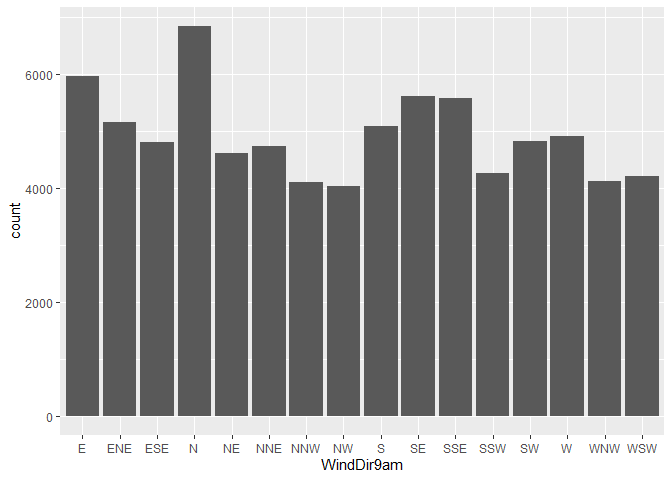
\includegraphics{Tarea1_files/figure-latex/unnamed-chunk-24-1.pdf}

Si representamos en un histograma la tabla de frecuencias absolutas
obtenida del colesterol de la muestra de pacientes obtenemos:

\begin{Shaded}
\begin{Highlighting}[]
\NormalTok{cortes }\OtherTok{=} \FunctionTok{seq}\NormalTok{(}\FunctionTok{min}\NormalTok{(chlstrl}\SpecialCharTok{$}\NormalTok{chol,}\AttributeTok{na.rm =} \ConstantTok{TRUE}\NormalTok{), }\FunctionTok{max}\NormalTok{(chlstrl}\SpecialCharTok{$}\NormalTok{chol,}\AttributeTok{na.rm =} \ConstantTok{TRUE}\NormalTok{), }\AttributeTok{length.out =} \DecValTok{12}\NormalTok{)}
\FunctionTok{ggplot}\NormalTok{(}\AttributeTok{data =} \FunctionTok{na.omit}\NormalTok{(chlstrl)) }\SpecialCharTok{+}
  \FunctionTok{geom\_histogram}\NormalTok{(}\AttributeTok{mapping =} \FunctionTok{aes}\NormalTok{(chol), }\AttributeTok{breaks =}\NormalTok{ cortes,}
                 \AttributeTok{fill =} \StringTok{"coral2"}\NormalTok{, }\AttributeTok{color=}\StringTok{"black"}\NormalTok{)}
\end{Highlighting}
\end{Shaded}

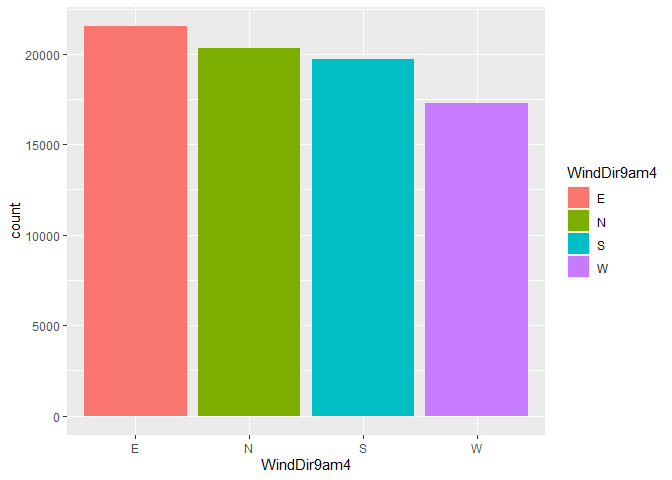
\includegraphics{Tarea1_files/figure-latex/unnamed-chunk-25-1.pdf}

Mientras que si representamos de forma conjunta la curva de densidad
junto con el histograma (pero representando las frecuencias relativas)
tenemos:

\begin{Shaded}
\begin{Highlighting}[]
\FunctionTok{ggplot}\NormalTok{(}\FunctionTok{na.omit}\NormalTok{(chlstrl), }\FunctionTok{aes}\NormalTok{(}\AttributeTok{x =}\NormalTok{ chol)) }\SpecialCharTok{+}
  \FunctionTok{geom\_histogram}\NormalTok{(}\FunctionTok{aes}\NormalTok{(}\AttributeTok{x =}\NormalTok{ chol,}\AttributeTok{y=}\FunctionTok{stat}\NormalTok{(density)),}
                 \AttributeTok{breaks =}\NormalTok{ cortes, }\AttributeTok{fill =} \StringTok{"coral2"}\NormalTok{, }\AttributeTok{color=}\StringTok{"black"}\NormalTok{)  }\SpecialCharTok{+}
  \FunctionTok{geom\_density}\NormalTok{(}\AttributeTok{mapping =} \FunctionTok{aes}\NormalTok{(chol),}\AttributeTok{color=}\StringTok{"darkslategrey"}\NormalTok{, }\AttributeTok{size=}\FloatTok{1.5}\NormalTok{)}
\end{Highlighting}
\end{Shaded}

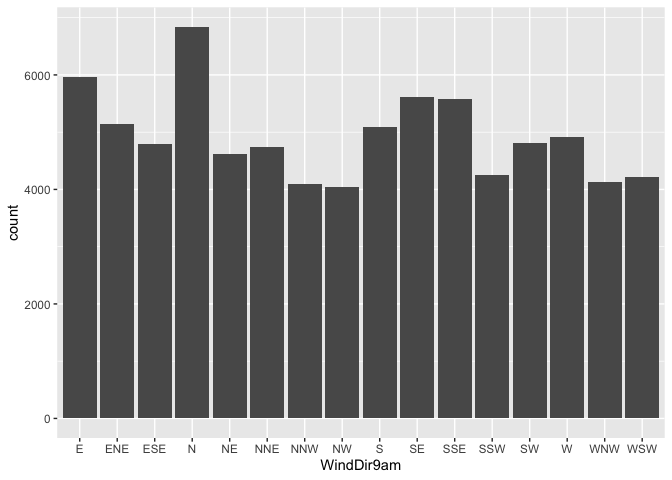
\includegraphics{Tarea1_files/figure-latex/unnamed-chunk-26-1.pdf}

Por último, para terminar de realizar el análisis exploratorio,
realizamos un \emph{violinplot}, en el que se nos brinda de información
del un diagrama de cajas además de disponer de curva de densidad y la
diospersión de los puntos:

\begin{Shaded}
\begin{Highlighting}[]
\FunctionTok{ggplot}\NormalTok{(}\FunctionTok{na.omit}\NormalTok{(chlstrl)) }\SpecialCharTok{+}
  \FunctionTok{geom\_violin}\NormalTok{(}\AttributeTok{mapping =} \FunctionTok{aes}\NormalTok{(}\AttributeTok{x=}\DecValTok{0}\NormalTok{, }\AttributeTok{y =}\NormalTok{ chol)) }\SpecialCharTok{+} \FunctionTok{scale\_x\_discrete}\NormalTok{(}\AttributeTok{breaks =} \FunctionTok{c}\NormalTok{()) }\SpecialCharTok{+}
  \FunctionTok{geom\_boxplot}\NormalTok{(}\AttributeTok{mapping =} \FunctionTok{aes}\NormalTok{(}\AttributeTok{y =}\NormalTok{ chol), }\AttributeTok{fill=}\StringTok{"coral2"}\NormalTok{) }\SpecialCharTok{+}
  \FunctionTok{geom\_jitter}\NormalTok{(}\FunctionTok{aes}\NormalTok{(}\AttributeTok{x=}\DecValTok{0}\NormalTok{, }\AttributeTok{y =}\NormalTok{ chol),}\AttributeTok{position =} \FunctionTok{position\_jitter}\NormalTok{(}\AttributeTok{w=}\FloatTok{0.05}\NormalTok{, }\AttributeTok{h=} \DecValTok{0}\NormalTok{), }\AttributeTok{col=}\StringTok{"darkslategrey"}\NormalTok{)}
\end{Highlighting}
\end{Shaded}

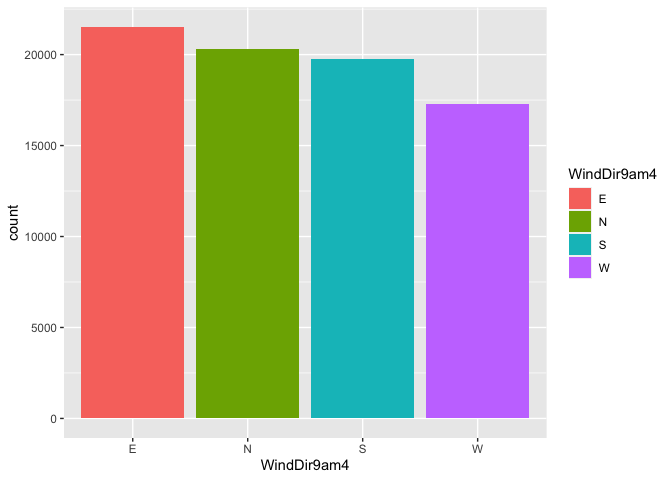
\includegraphics{Tarea1_files/figure-latex/unnamed-chunk-27-1.pdf}

Por otro lado tenemos como ejemplo de una variable categórica o factor
es la columna \texttt{gender}. Por defecto, cuando hemos importado la
tabla, la columna \texttt{gender} se ha guardado como \texttt{string}.
Por tanto primero debemos cambiar el tipo de la columna \texttt{gender}
a factor.

\begin{Shaded}
\begin{Highlighting}[]
\NormalTok{chlstrl}\SpecialCharTok{$}\NormalTok{gender}\OtherTok{=}\FunctionTok{factor}\NormalTok{(chlstrl}\SpecialCharTok{$}\NormalTok{gender)}
\end{Highlighting}
\end{Shaded}

\begin{Shaded}
\begin{Highlighting}[]
\FunctionTok{class}\NormalTok{(chlstrl}\SpecialCharTok{$}\NormalTok{gender)}
\end{Highlighting}
\end{Shaded}

\begin{verbatim}
## [1] "factor"
\end{verbatim}

Para saber cuántos hombres y mujeres en la muestra usamos la tabla de
frecuencias absolutas:

\begin{Shaded}
\begin{Highlighting}[]
\FunctionTok{table}\NormalTok{(chlstrl}\SpecialCharTok{$}\NormalTok{gender)}
\end{Highlighting}
\end{Shaded}

\begin{verbatim}
## 
## female   male 
##    234    169
\end{verbatim}

o una tabla de frecuencias relativas, que nos dice el porcentaje de
hombres y mujeres en tanto por 1. Esto se debe a que trabajamos con
factores dicotómicos.

\begin{Shaded}
\begin{Highlighting}[]
\FunctionTok{prop.table}\NormalTok{(}\FunctionTok{table}\NormalTok{(chlstrl}\SpecialCharTok{$}\NormalTok{gender))}
\end{Highlighting}
\end{Shaded}

\begin{verbatim}
## 
##    female      male 
## 0.5806452 0.4193548
\end{verbatim}

Podemos usar un diagrama de barras para representar una tabla de
frecuencias absolutas:

\begin{Shaded}
\begin{Highlighting}[]
\FunctionTok{ggplot}\NormalTok{(chlstrl) }\SpecialCharTok{+}
  \FunctionTok{geom\_bar}\NormalTok{(}\AttributeTok{mapping =} \FunctionTok{aes}\NormalTok{(}\AttributeTok{x =}\NormalTok{ gender), }\AttributeTok{fill=} \FunctionTok{c}\NormalTok{(}\StringTok{"coral"}\NormalTok{,}\StringTok{"grey"}\NormalTok{))}
\end{Highlighting}
\end{Shaded}

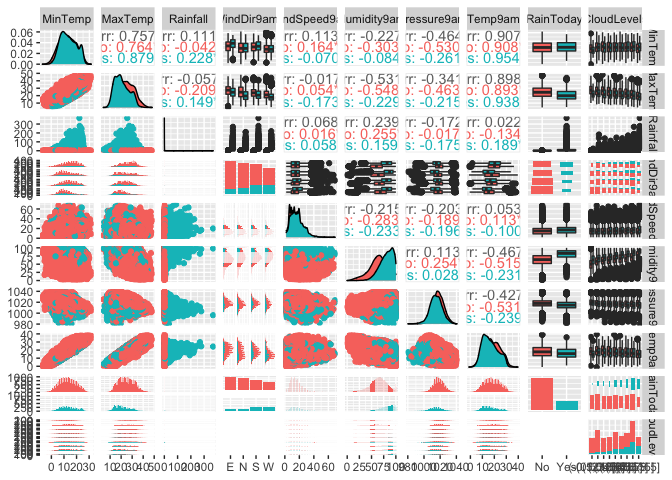
\includegraphics{Tarea1_files/figure-latex/unnamed-chunk-32-1.pdf} Dado
que estamos interesados en trabajar en el sistema internacional, SI,
realizamos el siguiente comando para cambiar las unidades de la altura,
\texttt{height}, y del peso, \texttt{weight}. Con \texttt{mutate()}
reemplazamos las columnas \texttt{height} y \texttt{weight} por las
versiones en el Sistema Internacional.

\begin{Shaded}
\begin{Highlighting}[]
\NormalTok{chlstrl }\SpecialCharTok{\%\textgreater{}\%} \FunctionTok{mutate}\NormalTok{(}\AttributeTok{height=}\NormalTok{height}\SpecialCharTok{*}\FloatTok{0.0254}\NormalTok{,}\AttributeTok{weight=}\NormalTok{weight}\SpecialCharTok{*}\FloatTok{0.454}\NormalTok{) }\OtherTok{{-}\textgreater{}}\NormalTok{ chlstrlSI}
\end{Highlighting}
\end{Shaded}

\begin{Shaded}
\begin{Highlighting}[]
\FunctionTok{head}\NormalTok{ (chlstrlSI)}
\end{Highlighting}
\end{Shaded}

\begin{verbatim}
## # A tibble: 6 x 7
##    chol   age gender height weight waist   hip
##   <dbl> <dbl> <fct>   <dbl>  <dbl> <dbl> <dbl>
## 1   203    46 female   1.57   54.9    29    38
## 2   165    29 female   1.63   99.0    46    48
## 3   228    58 female   1.55  116.     49    57
## 4    78    67 male     1.70   54.0    33    38
## 5   249    64 male     1.73   83.1    44    41
## 6   248    34 male     1.80   86.3    36    42
\end{verbatim}

Usando el comando \texttt{mutate()} creamos la columna \texttt{BMI} (ya
que no existe inicialmente la columna \texttt{BMI}, al usar
\texttt{mutate()} se crea)

\begin{Shaded}
\begin{Highlighting}[]
\NormalTok{chlstrlSI }\SpecialCharTok{\%\textgreater{}\%}
  \FunctionTok{mutate}\NormalTok{(}\StringTok{"BMI"} \OtherTok{=}\NormalTok{ weight}\SpecialCharTok{/}\NormalTok{(height)}\SpecialCharTok{\^{}}\DecValTok{2}\NormalTok{) }\OtherTok{{-}\textgreater{}}\NormalTok{ chlstrlSI}
\FunctionTok{head}\NormalTok{ (chlstrlSI)}
\end{Highlighting}
\end{Shaded}

\begin{verbatim}
## # A tibble: 6 x 8
##    chol   age gender height weight waist   hip   BMI
##   <dbl> <dbl> <fct>   <dbl>  <dbl> <dbl> <dbl> <dbl>
## 1   203    46 female   1.57   54.9    29    38  22.2
## 2   165    29 female   1.63   99.0    46    48  37.5
## 3   228    58 female   1.55  116.     49    57  48.4
## 4    78    67 male     1.70   54.0    33    38  18.7
## 5   249    64 male     1.73   83.1    44    41  27.8
## 6   248    34 male     1.80   86.3    36    42  26.5
\end{verbatim}

Usando el comando \texttt{cut()} creamos un vector de factores,
\texttt{ageGroup}, dividiendo las edades en tres grupos.

\begin{Shaded}
\begin{Highlighting}[]
\NormalTok{ageGroup}\OtherTok{=}\FunctionTok{cut}\NormalTok{(chlstrlSI}\SpecialCharTok{$}\NormalTok{age, }\AttributeTok{breaks =} \FunctionTok{seq}\NormalTok{(}\DecValTok{10}\NormalTok{,}\DecValTok{100}\NormalTok{,}\DecValTok{30}\NormalTok{))}
\FunctionTok{head}\NormalTok{(ageGroup)}
\end{Highlighting}
\end{Shaded}

\begin{verbatim}
## [1] (40,70] (10,40] (40,70] (40,70] (40,70] (10,40]
## Levels: (10,40] (40,70] (70,100]
\end{verbatim}

Añadimos este vector a la tabla \texttt{chlstrlSI}:

\begin{Shaded}
\begin{Highlighting}[]
\NormalTok{chlstrlSI }\SpecialCharTok{\%\textgreater{}\%} \FunctionTok{mutate}\NormalTok{(ageGroup) }\OtherTok{{-}\textgreater{}}\NormalTok{ chlstrlSI}
\FunctionTok{head}\NormalTok{ (chlstrlSI)}
\end{Highlighting}
\end{Shaded}

\begin{verbatim}
## # A tibble: 6 x 9
##    chol   age gender height weight waist   hip   BMI ageGroup
##   <dbl> <dbl> <fct>   <dbl>  <dbl> <dbl> <dbl> <dbl> <fct>   
## 1   203    46 female   1.57   54.9    29    38  22.2 (40,70] 
## 2   165    29 female   1.63   99.0    46    48  37.5 (10,40] 
## 3   228    58 female   1.55  116.     49    57  48.4 (40,70] 
## 4    78    67 male     1.70   54.0    33    38  18.7 (40,70] 
## 5   249    64 male     1.73   83.1    44    41  27.8 (40,70] 
## 6   248    34 male     1.80   86.3    36    42  26.5 (10,40]
\end{verbatim}

Para saber la media del nivel de colesterol y de BMI de las mujeres en
cada uno de los grupos de edad. Usamos \texttt{group\_by()} para agrupar
por grupos de edad, \texttt{group\_by}, el comando \texttt{filter()}
para decir que sean mujeres, y con el comando \texttt{summarise()}
creamos un nuevo \emph{data.frame} donde calculamos la media del
colesterol y de la media.

\begin{Shaded}
\begin{Highlighting}[]
\NormalTok{chlstrlSI }\SpecialCharTok{\%\textgreater{}\%} \FunctionTok{group\_by}\NormalTok{(ageGroup) }\SpecialCharTok{\%\textgreater{}\%} \FunctionTok{filter}\NormalTok{(gender}\SpecialCharTok{==}\StringTok{"female"}\NormalTok{)  }\SpecialCharTok{\%\textgreater{}\%}
  \FunctionTok{summarise}\NormalTok{(}\AttributeTok{MediaChol=}\FunctionTok{mean}\NormalTok{(chol,}\AttributeTok{na.rm =} \ConstantTok{TRUE}\NormalTok{), }\AttributeTok{MediaBMI=}\FunctionTok{mean}\NormalTok{(BMI,}\AttributeTok{na.rm =} \ConstantTok{TRUE}\NormalTok{))}
\end{Highlighting}
\end{Shaded}

\begin{verbatim}
## # A tibble: 3 x 3
##   ageGroup MediaChol MediaBMI
##   <fct>        <dbl>    <dbl>
## 1 (10,40]       189.     30.5
## 2 (40,70]       221.     30.3
## 3 (70,100]      230.     29.4
\end{verbatim}

\hypertarget{ejercicio-2}{%
\subsubsection{Ejercicio 2}\label{ejercicio-2}}

En primer lugar creamos el vector \texttt{x} de números enteros no nulos
dado como ejemplo y un vector \texttt{y} que genera vectores aleatorios
enteros no nulos.

\begin{Shaded}
\begin{Highlighting}[]
\NormalTok{x}\OtherTok{=}\FunctionTok{c}\NormalTok{(}\SpecialCharTok{{-}}\DecValTok{12}\NormalTok{,}\SpecialCharTok{{-}}\DecValTok{19}\NormalTok{,}\DecValTok{9}\NormalTok{,}\SpecialCharTok{{-}}\DecValTok{13}\NormalTok{,}\SpecialCharTok{{-}}\DecValTok{14}\NormalTok{,}\SpecialCharTok{{-}}\DecValTok{17}\NormalTok{,}\DecValTok{8}\NormalTok{,}\SpecialCharTok{{-}}\DecValTok{19}\NormalTok{,}\SpecialCharTok{{-}}\DecValTok{10}\NormalTok{)}
\NormalTok{y}\OtherTok{=}\FunctionTok{sample}\NormalTok{(}\FunctionTok{c}\NormalTok{(}\SpecialCharTok{{-}}\DecValTok{20}\SpecialCharTok{:{-}}\DecValTok{1}\NormalTok{,}\DecValTok{1}\SpecialCharTok{:}\DecValTok{20}\NormalTok{),}\DecValTok{9}\NormalTok{,}\AttributeTok{replace =} \ConstantTok{TRUE}\NormalTok{)}
\end{Highlighting}
\end{Shaded}

\begin{verbatim}
## [1] -12 -19   9 -13 -14 -17
\end{verbatim}

\begin{Shaded}
\begin{Highlighting}[]
\NormalTok{y}\OtherTok{=}\FunctionTok{sample}\NormalTok{(}\FunctionTok{c}\NormalTok{(}\SpecialCharTok{{-}}\DecValTok{20}\SpecialCharTok{:{-}}\DecValTok{1}\NormalTok{,}\DecValTok{1}\SpecialCharTok{:}\DecValTok{20}\NormalTok{),}\DecValTok{9}\NormalTok{,}\AttributeTok{replace =} \ConstantTok{TRUE}\NormalTok{)}
\end{Highlighting}
\end{Shaded}

\begin{verbatim}
## [1]   5 -13  -6  14  -8 -11
\end{verbatim}

Ahora, creamos una función que calcula cuantos cambios de signo tiene el
vector:

\begin{Shaded}
\begin{Highlighting}[]
\NormalTok{cambiosSigno}\OtherTok{=}\ControlFlowTok{function}\NormalTok{(x)\{}
\NormalTok{i}\OtherTok{=}\DecValTok{0}
  \ControlFlowTok{for}\NormalTok{(k }\ControlFlowTok{in} \FunctionTok{seq}\NormalTok{(}\FunctionTok{length}\NormalTok{(x)}\SpecialCharTok{{-}}\DecValTok{1}\NormalTok{))\{}
    \ControlFlowTok{if}\NormalTok{( x[k]}\SpecialCharTok{*}\NormalTok{x[k}\SpecialCharTok{+}\DecValTok{1}\NormalTok{]}\SpecialCharTok{\textless{}}\DecValTok{0}\NormalTok{ )\{}
\NormalTok{      i}\OtherTok{=}\NormalTok{i}\SpecialCharTok{+}\DecValTok{1}
\NormalTok{    \}}
\NormalTok{  \}}
\FunctionTok{return}\NormalTok{(i)}
\NormalTok{\}}
\end{Highlighting}
\end{Shaded}

Y la funciónb que calcula en que posiciones se han producido los cambios
de signo y devuelve un mensaje cuando no se ha producido ningún cambio:

\begin{Shaded}
\begin{Highlighting}[]
\NormalTok{cambiosSignoPos}\OtherTok{=}\ControlFlowTok{function}\NormalTok{(x)\{}
\NormalTok{pos}\OtherTok{=}\FunctionTok{c}\NormalTok{()}
  \ControlFlowTok{for}\NormalTok{(k }\ControlFlowTok{in} \FunctionTok{seq}\NormalTok{(}\FunctionTok{length}\NormalTok{(x)}\SpecialCharTok{{-}}\DecValTok{1}\NormalTok{))\{}
    \ControlFlowTok{if}\NormalTok{( x[k]}\SpecialCharTok{*}\NormalTok{x[k}\SpecialCharTok{+}\DecValTok{1}\NormalTok{]}\SpecialCharTok{\textless{}}\DecValTok{0}\NormalTok{ )\{}
\NormalTok{      pos}\OtherTok{=}\FunctionTok{append}\NormalTok{(pos,k}\SpecialCharTok{+}\DecValTok{1}\NormalTok{)}
\NormalTok{    \}}
\NormalTok{  \}}
  \ControlFlowTok{if}\NormalTok{( }\FunctionTok{is.null}\NormalTok{(pos) }\SpecialCharTok{==} \ConstantTok{TRUE}\NormalTok{)\{}
    \FunctionTok{print}\NormalTok{(}\StringTok{"No hay ningún cambio de signo"}\NormalTok{)}
\NormalTok{    \}}\ControlFlowTok{else}\NormalTok{\{}
      \FunctionTok{return}\NormalTok{(pos)}
\NormalTok{    \}}
\NormalTok{\}}
\end{Highlighting}
\end{Shaded}

\hypertarget{ejercicio-3}{%
\subsubsection{Ejercicio 3}\label{ejercicio-3}}

Queremos replicar las gráficas que aparecen en la sección 3 y 5 del
libro R for Data Science. Guardamos cada gráfica en una variable y luego
usamos el comando \texttt{grid.arrange}.

\begin{Shaded}
\begin{Highlighting}[]
\FunctionTok{library}\NormalTok{(gridExtra)}
\end{Highlighting}
\end{Shaded}

\begin{Shaded}
\begin{Highlighting}[]
\FunctionTok{ggplot}\NormalTok{(}\AttributeTok{data =}\NormalTok{ mpg, }\AttributeTok{mapping =} \FunctionTok{aes}\NormalTok{(}\AttributeTok{x =}\NormalTok{ displ, }\AttributeTok{y =}\NormalTok{ hwy)) }\SpecialCharTok{+}
  \FunctionTok{geom\_point}\NormalTok{() }\SpecialCharTok{+}
  \FunctionTok{geom\_smooth}\NormalTok{(}\AttributeTok{se =} \ConstantTok{FALSE}\NormalTok{,}\AttributeTok{method =} \StringTok{\textquotesingle{}loess\textquotesingle{}}\NormalTok{,}\AttributeTok{formula =}\NormalTok{y }\SpecialCharTok{\textasciitilde{}}\NormalTok{ x) }\OtherTok{{-}\textgreater{}}\NormalTok{ g1}
\FunctionTok{ggplot}\NormalTok{(}\AttributeTok{data =}\NormalTok{ mpg, }\AttributeTok{mapping =} \FunctionTok{aes}\NormalTok{(}\AttributeTok{x =}\NormalTok{ displ, }\AttributeTok{y =}\NormalTok{ hwy, }\AttributeTok{group =}\NormalTok{ drv)) }\SpecialCharTok{+}
  \FunctionTok{geom\_point}\NormalTok{() }\SpecialCharTok{+}
  \FunctionTok{geom\_smooth}\NormalTok{(}\AttributeTok{se =} \ConstantTok{FALSE}\NormalTok{,}\AttributeTok{method =} \StringTok{\textquotesingle{}loess\textquotesingle{}}\NormalTok{,}\AttributeTok{formula =}\NormalTok{y }\SpecialCharTok{\textasciitilde{}}\NormalTok{ x) }\OtherTok{{-}\textgreater{}}\NormalTok{ g2}
\FunctionTok{ggplot}\NormalTok{(}\AttributeTok{data =}\NormalTok{ mpg, }\AttributeTok{mapping =} \FunctionTok{aes}\NormalTok{(}\AttributeTok{x =}\NormalTok{ displ, }\AttributeTok{y =}\NormalTok{ hwy, }\AttributeTok{colour =}\NormalTok{ drv)) }\SpecialCharTok{+}
  \FunctionTok{geom\_point}\NormalTok{() }\SpecialCharTok{+}
  \FunctionTok{geom\_smooth}\NormalTok{(}\AttributeTok{se =} \ConstantTok{FALSE}\NormalTok{,}\AttributeTok{method =} \StringTok{\textquotesingle{}loess\textquotesingle{}}\NormalTok{,}\AttributeTok{formula =}\NormalTok{y }\SpecialCharTok{\textasciitilde{}}\NormalTok{ x) }\OtherTok{{-}\textgreater{}}\NormalTok{ g3}
\FunctionTok{ggplot}\NormalTok{() }\SpecialCharTok{+}
  \FunctionTok{geom\_point}\NormalTok{(}\AttributeTok{data =}\NormalTok{ mpg, }\AttributeTok{mapping =} \FunctionTok{aes}\NormalTok{(}\AttributeTok{x =}\NormalTok{ displ, }\AttributeTok{y =}\NormalTok{ hwy, }\AttributeTok{colour =}\NormalTok{ drv)) }\SpecialCharTok{+}
  \FunctionTok{geom\_smooth}\NormalTok{(}\AttributeTok{data =}\NormalTok{ mpg, }\AttributeTok{mapping =} \FunctionTok{aes}\NormalTok{(}\AttributeTok{x =}\NormalTok{ displ, }\AttributeTok{y =}\NormalTok{ hwy),}\AttributeTok{se =} \ConstantTok{FALSE}\NormalTok{,}\AttributeTok{method =} \StringTok{\textquotesingle{}loess\textquotesingle{}}\NormalTok{,}\AttributeTok{formula =}\NormalTok{y }\SpecialCharTok{\textasciitilde{}}\NormalTok{ x) }\OtherTok{{-}\textgreater{}}\NormalTok{ g4}
\FunctionTok{ggplot}\NormalTok{() }\SpecialCharTok{+}
  \FunctionTok{geom\_point}\NormalTok{(}\AttributeTok{data =}\NormalTok{ mpg, }\AttributeTok{mapping =} \FunctionTok{aes}\NormalTok{(}\AttributeTok{x =}\NormalTok{ displ, }\AttributeTok{y =}\NormalTok{ hwy, }\AttributeTok{colour =}\NormalTok{ drv)) }\SpecialCharTok{+}
  \FunctionTok{geom\_smooth}\NormalTok{(}\AttributeTok{data =}\NormalTok{ mpg, }\AttributeTok{mapping =} \FunctionTok{aes}\NormalTok{(}\AttributeTok{x =}\NormalTok{ displ, }\AttributeTok{y =}\NormalTok{ hwy, }\AttributeTok{linetype =}\NormalTok{ drv),}\AttributeTok{se =} \ConstantTok{FALSE}\NormalTok{,}\AttributeTok{method =} \StringTok{\textquotesingle{}loess\textquotesingle{}}\NormalTok{,}\AttributeTok{formula =}\NormalTok{y }\SpecialCharTok{\textasciitilde{}}\NormalTok{ x) }\OtherTok{{-}\textgreater{}}\NormalTok{ g5}
\FunctionTok{ggplot}\NormalTok{(mpg, }\FunctionTok{aes}\NormalTok{(}\AttributeTok{x =}\NormalTok{ displ, }\AttributeTok{y =}\NormalTok{ hwy)) }\SpecialCharTok{+}
  \FunctionTok{geom\_point}\NormalTok{(}\AttributeTok{size =} \DecValTok{4}\NormalTok{, }\AttributeTok{color =} \StringTok{"white"}\NormalTok{) }\SpecialCharTok{+}
  \FunctionTok{geom\_point}\NormalTok{(}\FunctionTok{aes}\NormalTok{(}\AttributeTok{colour =}\NormalTok{ drv)) }\OtherTok{{-}\textgreater{}}\NormalTok{ g6}
\FunctionTok{grid.arrange}\NormalTok{(g1, g2, g3, g4,g5,g6, }\AttributeTok{nrow =} \DecValTok{3}\NormalTok{)}
\end{Highlighting}
\end{Shaded}

\includegraphics{Tarea1_files/figure-latex/unnamed-chunk-46-1.pdf}

Ahora realizaremos una serie de consultas que realizaremos con el
comando \texttt{filter()}. Primero cargamos la libreria necesaria:

\begin{Shaded}
\begin{Highlighting}[]
\FunctionTok{library}\NormalTok{(nycflights13)}
\end{Highlighting}
\end{Shaded}

Vuelos que tengan retraso en la hora de llegada de dos horas o más:

\begin{Shaded}
\begin{Highlighting}[]
\FunctionTok{filter}\NormalTok{(flights, arr\_delay}\SpecialCharTok{\textgreater{}=}\DecValTok{120}\NormalTok{ )}
\end{Highlighting}
\end{Shaded}

\begin{verbatim}
## # A tibble: 10,200 x 19
##     year month   day dep_time sched_dep_time dep_delay arr_time sched_arr_time
##    <int> <int> <int>    <int>          <int>     <dbl>    <int>          <int>
##  1  2013     1     1      811            630       101     1047            830
##  2  2013     1     1      848           1835       853     1001           1950
##  3  2013     1     1      957            733       144     1056            853
##  4  2013     1     1     1114            900       134     1447           1222
##  5  2013     1     1     1505           1310       115     1638           1431
##  6  2013     1     1     1525           1340       105     1831           1626
##  7  2013     1     1     1549           1445        64     1912           1656
##  8  2013     1     1     1558           1359       119     1718           1515
##  9  2013     1     1     1732           1630        62     2028           1825
## 10  2013     1     1     1803           1620       103     2008           1750
## # ... with 10,190 more rows, and 11 more variables: arr_delay <dbl>,
## #   carrier <chr>, flight <int>, tailnum <chr>, origin <chr>, dest <chr>,
## #   air_time <dbl>, distance <dbl>, hour <dbl>, minute <dbl>, time_hour <dttm>
\end{verbatim}

Vuelos que volaron a Houston:

\begin{Shaded}
\begin{Highlighting}[]
\FunctionTok{filter}\NormalTok{(flights, dest }\SpecialCharTok{==} \StringTok{"IAH"} \SpecialCharTok{|}\NormalTok{ dest }\SpecialCharTok{==} \StringTok{"HOU"}\NormalTok{)}
\end{Highlighting}
\end{Shaded}

\begin{verbatim}
## # A tibble: 9,313 x 19
##     year month   day dep_time sched_dep_time dep_delay arr_time sched_arr_time
##    <int> <int> <int>    <int>          <int>     <dbl>    <int>          <int>
##  1  2013     1     1      517            515         2      830            819
##  2  2013     1     1      533            529         4      850            830
##  3  2013     1     1      623            627        -4      933            932
##  4  2013     1     1      728            732        -4     1041           1038
##  5  2013     1     1      739            739         0     1104           1038
##  6  2013     1     1      908            908         0     1228           1219
##  7  2013     1     1     1028           1026         2     1350           1339
##  8  2013     1     1     1044           1045        -1     1352           1351
##  9  2013     1     1     1114            900       134     1447           1222
## 10  2013     1     1     1205           1200         5     1503           1505
## # ... with 9,303 more rows, and 11 more variables: arr_delay <dbl>,
## #   carrier <chr>, flight <int>, tailnum <chr>, origin <chr>, dest <chr>,
## #   air_time <dbl>, distance <dbl>, hour <dbl>, minute <dbl>, time_hour <dttm>
\end{verbatim}

Vuelos cuya operadora fue United, American o Delta:

\begin{Shaded}
\begin{Highlighting}[]
\FunctionTok{filter}\NormalTok{(flights, carrier }\SpecialCharTok{==} \StringTok{"UA"} \SpecialCharTok{|}\NormalTok{ carrier }\SpecialCharTok{==} \StringTok{"AA"} \SpecialCharTok{|}\NormalTok{ carrier }\SpecialCharTok{==} \StringTok{"DL"}\NormalTok{)}
\end{Highlighting}
\end{Shaded}

\begin{verbatim}
## # A tibble: 139,504 x 19
##     year month   day dep_time sched_dep_time dep_delay arr_time sched_arr_time
##    <int> <int> <int>    <int>          <int>     <dbl>    <int>          <int>
##  1  2013     1     1      517            515         2      830            819
##  2  2013     1     1      533            529         4      850            830
##  3  2013     1     1      542            540         2      923            850
##  4  2013     1     1      554            600        -6      812            837
##  5  2013     1     1      554            558        -4      740            728
##  6  2013     1     1      558            600        -2      753            745
##  7  2013     1     1      558            600        -2      924            917
##  8  2013     1     1      558            600        -2      923            937
##  9  2013     1     1      559            600        -1      941            910
## 10  2013     1     1      559            600        -1      854            902
## # ... with 139,494 more rows, and 11 more variables: arr_delay <dbl>,
## #   carrier <chr>, flight <int>, tailnum <chr>, origin <chr>, dest <chr>,
## #   air_time <dbl>, distance <dbl>, hour <dbl>, minute <dbl>, time_hour <dttm>
\end{verbatim}

Vuelos que se realizaron en verano:

\begin{Shaded}
\begin{Highlighting}[]
\FunctionTok{filter}\NormalTok{(flights, month }\SpecialCharTok{==} \DecValTok{6} \SpecialCharTok{|}\NormalTok{ month }\SpecialCharTok{==} \DecValTok{7} \SpecialCharTok{|}\NormalTok{ month }\SpecialCharTok{==} \DecValTok{8}\NormalTok{)}
\end{Highlighting}
\end{Shaded}

\begin{verbatim}
## # A tibble: 86,995 x 19
##     year month   day dep_time sched_dep_time dep_delay arr_time sched_arr_time
##    <int> <int> <int>    <int>          <int>     <dbl>    <int>          <int>
##  1  2013     6     1        2           2359         3      341            350
##  2  2013     6     1      451            500        -9      624            640
##  3  2013     6     1      506            515        -9      715            800
##  4  2013     6     1      534            545       -11      800            829
##  5  2013     6     1      538            545        -7      925            922
##  6  2013     6     1      539            540        -1      832            840
##  7  2013     6     1      546            600       -14      850            910
##  8  2013     6     1      551            600        -9      828            850
##  9  2013     6     1      552            600        -8      647            655
## 10  2013     6     1      553            600        -7      700            711
## # ... with 86,985 more rows, and 11 more variables: arr_delay <dbl>,
## #   carrier <chr>, flight <int>, tailnum <chr>, origin <chr>, dest <chr>,
## #   air_time <dbl>, distance <dbl>, hour <dbl>, minute <dbl>, time_hour <dttm>
\end{verbatim}

No salieron tarde pero llegaron más de dos horas tarde:

\begin{Shaded}
\begin{Highlighting}[]
\FunctionTok{filter}\NormalTok{(flights, dep\_delay}\SpecialCharTok{\textless{}=}\DecValTok{0}\NormalTok{ , arr\_delay}\SpecialCharTok{\textgreater{}=}\DecValTok{120}\NormalTok{)}
\end{Highlighting}
\end{Shaded}

\begin{verbatim}
## # A tibble: 29 x 19
##     year month   day dep_time sched_dep_time dep_delay arr_time sched_arr_time
##    <int> <int> <int>    <int>          <int>     <dbl>    <int>          <int>
##  1  2013     1    27     1419           1420        -1     1754           1550
##  2  2013    10     7     1350           1350         0     1736           1526
##  3  2013    10     7     1357           1359        -2     1858           1654
##  4  2013    10    16      657            700        -3     1258           1056
##  5  2013    11     1      658            700        -2     1329           1015
##  6  2013     3    18     1844           1847        -3       39           2219
##  7  2013     4    17     1635           1640        -5     2049           1845
##  8  2013     4    18      558            600        -2     1149            850
##  9  2013     4    18      655            700        -5     1213            950
## 10  2013     5    22     1827           1830        -3     2217           2010
## # ... with 19 more rows, and 11 more variables: arr_delay <dbl>, carrier <chr>,
## #   flight <int>, tailnum <chr>, origin <chr>, dest <chr>, air_time <dbl>,
## #   distance <dbl>, hour <dbl>, minute <dbl>, time_hour <dttm>
\end{verbatim}

Vuelos que se retrasaron por lo menos una hora en la salida, pero
recuperaron media hora:

\begin{Shaded}
\begin{Highlighting}[]
\FunctionTok{filter}\NormalTok{(flights, dep\_delay}\SpecialCharTok{{-}}\NormalTok{arr\_delay}\SpecialCharTok{\textless{}=}\DecValTok{30}\NormalTok{, dep\_delay}\SpecialCharTok{\textgreater{}=}\DecValTok{60}\NormalTok{)}
\end{Highlighting}
\end{Shaded}

\begin{verbatim}
## # A tibble: 24,958 x 19
##     year month   day dep_time sched_dep_time dep_delay arr_time sched_arr_time
##    <int> <int> <int>    <int>          <int>     <dbl>    <int>          <int>
##  1  2013     1     1      811            630       101     1047            830
##  2  2013     1     1      826            715        71     1136           1045
##  3  2013     1     1      848           1835       853     1001           1950
##  4  2013     1     1      957            733       144     1056            853
##  5  2013     1     1     1114            900       134     1447           1222
##  6  2013     1     1     1120            944        96     1331           1213
##  7  2013     1     1     1301           1150        71     1518           1345
##  8  2013     1     1     1337           1220        77     1649           1531
##  9  2013     1     1     1400           1250        70     1645           1502
## 10  2013     1     1     1505           1310       115     1638           1431
## # ... with 24,948 more rows, and 11 more variables: arr_delay <dbl>,
## #   carrier <chr>, flight <int>, tailnum <chr>, origin <chr>, dest <chr>,
## #   air_time <dbl>, distance <dbl>, hour <dbl>, minute <dbl>, time_hour <dttm>
\end{verbatim}

Salieron entre medianoche y las 6 AM:

\begin{Shaded}
\begin{Highlighting}[]
\FunctionTok{filter}\NormalTok{(flights, dep\_time}\SpecialCharTok{\textgreater{}=}\DecValTok{0} \SpecialCharTok{\&}\NormalTok{ dep\_time}\SpecialCharTok{\textless{}=}\DecValTok{600}\NormalTok{)}
\end{Highlighting}
\end{Shaded}

\begin{verbatim}
## # A tibble: 9,344 x 19
##     year month   day dep_time sched_dep_time dep_delay arr_time sched_arr_time
##    <int> <int> <int>    <int>          <int>     <dbl>    <int>          <int>
##  1  2013     1     1      517            515         2      830            819
##  2  2013     1     1      533            529         4      850            830
##  3  2013     1     1      542            540         2      923            850
##  4  2013     1     1      544            545        -1     1004           1022
##  5  2013     1     1      554            600        -6      812            837
##  6  2013     1     1      554            558        -4      740            728
##  7  2013     1     1      555            600        -5      913            854
##  8  2013     1     1      557            600        -3      709            723
##  9  2013     1     1      557            600        -3      838            846
## 10  2013     1     1      558            600        -2      753            745
## # ... with 9,334 more rows, and 11 more variables: arr_delay <dbl>,
## #   carrier <chr>, flight <int>, tailnum <chr>, origin <chr>, dest <chr>,
## #   air_time <dbl>, distance <dbl>, hour <dbl>, minute <dbl>, time_hour <dttm>
\end{verbatim}

\end{document}
